% AER-Article.tex for AEA last revised 22 June 2011
\documentclass[]{AEA}
\usepackage{amsmath}
\def\sym#1{\ifmmode^{#1}\else\(^{#1}\)\fi}
\usepackage{float} %設定圖片浮動位置的宏包
\usepackage{graphicx} %插入圖片
\usepackage{subfigure} %插入多圖時用子圖顯示
\usepackage{siunitx} % used for regression table
\usepackage{booktabs} % used for regression table
\usepackage{natbib}

\usepackage{xeCJK}
\setCJKmainfont{NotoSansCJKtc-Regular.otf}
%\setcitestyle{authoryear, round}


%%%%%% NOTE FROM OVERLEAF: The mathtime package is no longer publicly available nor distributed. We recommend using a different font package e.g. mathptmx if you'd like to use a Times font.
% \usepackage{mathptmx}

% The mathtime package uses a Times font instead of Computer Modern.
% Uncomment the line below if you wish to use the mathtime package:
%\usepackage[cmbold]{mathtime}
% Note that miktex, by default, configures the mathtime package to use commercial fonts
% which you may not have. If you would like to use mathtime but you are seeing error
% messages about missing fonts (mtex.pfb, mtsy.pfb, or rmtmi.pfb) then please see
% the technical support document at http://www.aeaweb.org/templates/technical_support.pdf
% for instructions on fixing this problem.

% Note: you may use either harvard or natbib (but not both) to provide a wider
% variety of citation commands than latex supports natively. See below.

% Uncomment the next line to use the harvard package with bibtex
\usepackage[abbr]{harvard}

% This command determines the leading (vertical space between lines) in draft mode
% with 1.5 corresponding to "double" spacing.

\draftSpacing{1.5}

\begin{document}


\title{How does Single Parent Family Affect Children's Human Capital Investment}
\shortTitle{Single Parent family effect}
\author{Yi Jie Wu, Xiang Jyun Jhang\thanks{Wu: Department of Economics, National Taiwan University, b08302129@ntu.edu.tw; Jhang: Department of Economics, National Taiwan University, b08303024@ntu.edu.tw.  We are sincerely grateful for comments and advices from prof. Tzu-Ting Yang}}
\date{\today}
\pubMonth{JULY}
\pubYear{2023}

\begin{abstract}
    We estimate the impact of living in the single parent family on the children's future educational attainment by using a comprehensive panel survey data on students in Taiwan (TEPS).  By conducting PDS method, it's found that the experience of living in single parent family will decrease the probability of attaining university degree by 2.6 percent, and master degree by 4.6 percents also.  We also finds that there is a gap between the probability for two different groups of sample, which we provides some evidence to show it is attributed to the Taiwan Educational Reform in 2000s.
\end{abstract}


\maketitle

\section{Introduction}

    Over the past decade, a bunch of literatures investigated the impact of family background on children's futrure performance. The influence of single parent family is also a popular subtopic. The general trend is that students from single parent families are scored lower than those from normal families.\cite{barajas2011} 

    \cite{krein1988} has shown that the the negative impact of single parent families intensify when the period students staying in this type of family is longer. \cite{pong2003} compared the math and science achievement of third and fourth graders across 11 countries, and the results indicate that there's significant nagative effect of single parent families in 9 countries, except Australia and New Zealand, since these two countries have the entire family policies, reduce the negative effect of single parent families.

    Most research focus on the impact on scores or GPA, while less research talk about the long-term socioeconomic outcomes, like the degree of education. \cite{bernardi2014} use several countries data and find that children in seperated family have lower probability of achieving the university degree. Moreover, children living in higher education level family are more affected by the divorce event. The probability of obtaining the University degree is significantly affected by single parent family and their parents' education level.

    So why the single parent family has negative effect on their children? \cite{pong2003} form a possible system. There're two possible channels: one is financial capital channel, the other is social capital channel. The first channel indicates that single parent families only have one income source, which is less stable than two parent families. The second channel is that single parent has less time to accompany children, the parent absense during the children's learning period might also have some negative effect.

    In this article, we are interested in the probability of getting the higher education degree. We will include the university degree and master degree as main dependent variables. Furthermore, because the top public universities in Taiwan have much resources and lower tuition, it is popular for students with higher grades to choose top public university.\citep{luoh2018} Thus, we'll also see the public university degree as a important dependent variables, and try to observe how the single parent families influence children's attainment of higher education degree.

    Our data shows that single parent families have quite different effect in different periods. For the group born later, single parent families always have significant negative impact on university, master, and public university degrees, while for the group born earlier, the negative effect is less pronounced. After showing the whole analysis, we'll give our explaination for these difference.

    The empirical results are presented in the following four parts: the second part is about our dataset; the third part describes how we build the model. the fourth part presents the empirical results for three main dependent variables and single parent families; the fifth part discusses our interpretation of the results and links them to the policy changes.
    


\section{Data and Sample} % first paragraph: how the sample is built from the dataset?

    The datasets we use are Taiwan Education Panel Survey (TEPS) and Taiwan Education Panel Survey and Beyond (TEPS-B), in which there are two groups of children being surveyed consistently from their schoold age (16-18) to their working age (25-30) and each contains roughly 20,000 samples. The former dataset contains the in-school performance and characteristics of each child by surveying on their parents, teacher of each subject and children themselves. The latter dataset contains the characteristics and working status after the children entered into the labor market, and tracking down the sample for several years.  In the whole dataset, there are two main groups of sample, senior high (SH) group and core population (CP) group (sometimes, we also call it NPCP group since there are some newly added sample in this group).  The only difference between these two groups is the year of birth: the birth for SH group is 1984-1985, but for CP group is 1988-1989.  However, this unnoticed difference leads us to divide them into two groups and perform the same analysis, and it shows us some unexpected results which will be revealed later.

    Since our aim is to estimate the causal effect of living in single parent family on children's future educational attainment, we start by clarifying the condition of living in single parent family.  As we restricted the period we concerned to high-school age, which is usually the rapidly changing period in life, we define our treatment variable as below:

    \[
        \textit{SP}_i =
        \left\{\begin{aligned}
        &1,\quad\text{if child $i$ once under SP family in senior high} \\
        &0,\quad\text{o.w}
        \end{aligned}\right.
    \]

    On the other hand, to identify the children's future educational attainment, we choose three different kinds of outcome variable, which are \textbf{university degree, master degree and public university}.   The first and second variable are straight-forward, that is whether they obtain the degree when the data are recoreded.  The last one is more about the academic performance measured at the end of their high school age, since the entrance of public university is more competitive than private ones.  All these covariates are defined by using the data from TEPS-B, which provides the educational degree and whether the children enter job market after they're above 24-25 years old, so we can identify their final educational attainment.  
    
    To grasp the intuition, we present the ratio of each outcome variable by living in single parent family or not in figure 1.  It's not surprising that in both group, the educational outcome of children living in single parent family is lower than those who are not.  Besides, one more thing catches our attention is the significantly increasing trend in the public university, which reflecting the policy changes which we will focus on in later analysis.

    \begin{figure}
        \caption{Ratio of different outcome variables for each group}
        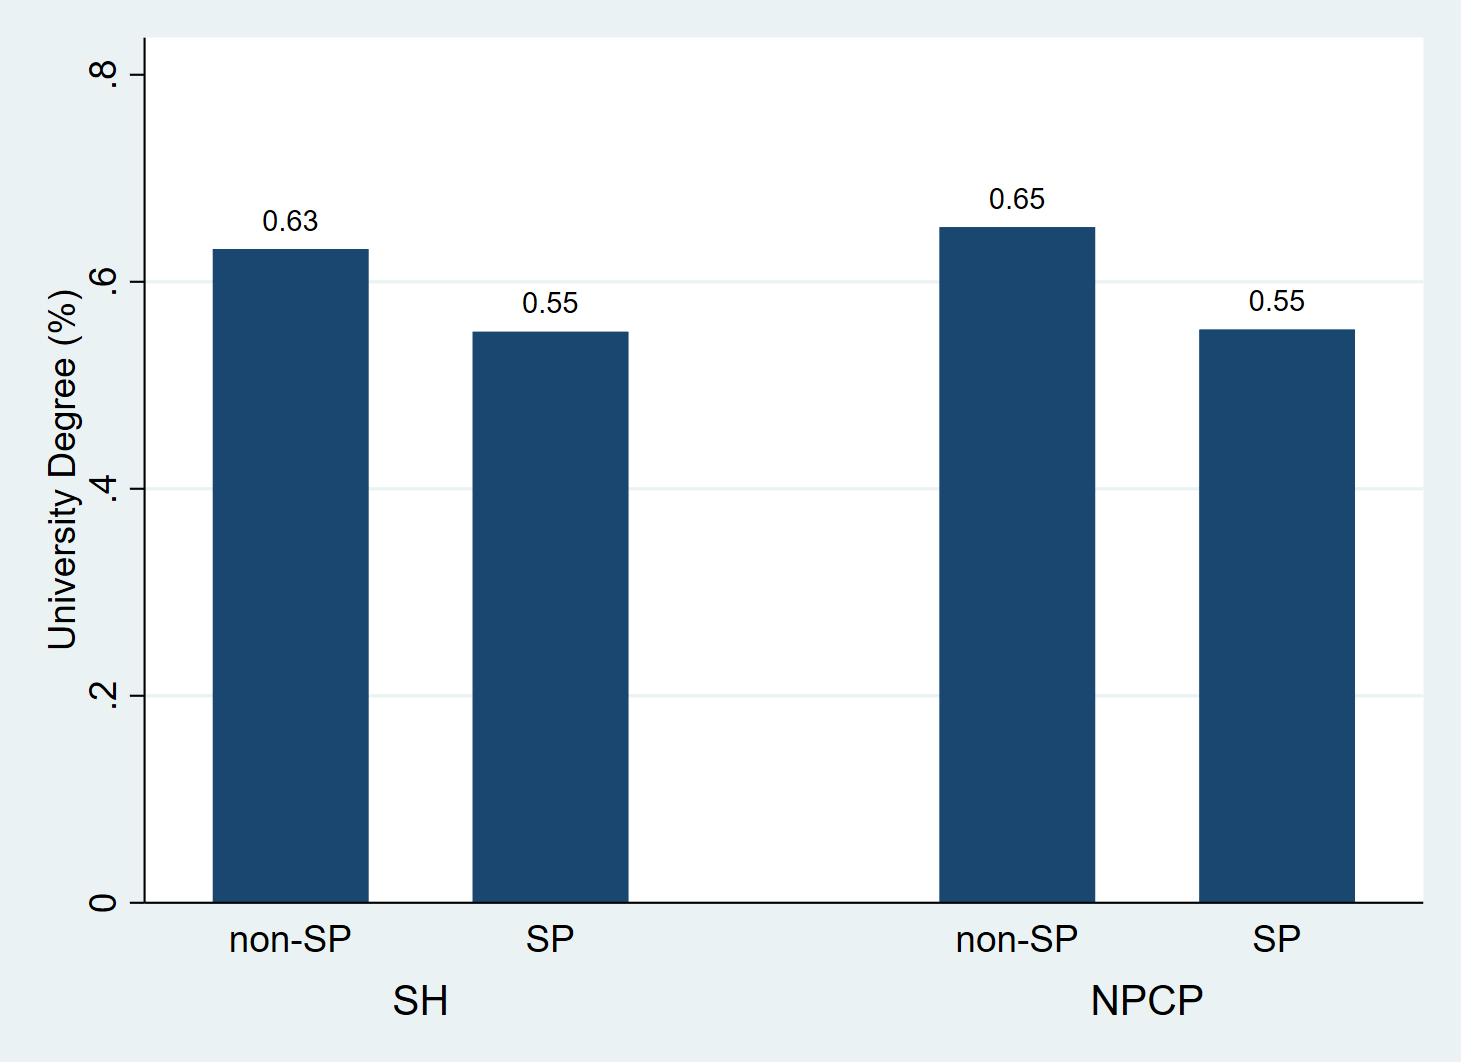
\includegraphics[scale=0.13]{university_sp.png}
        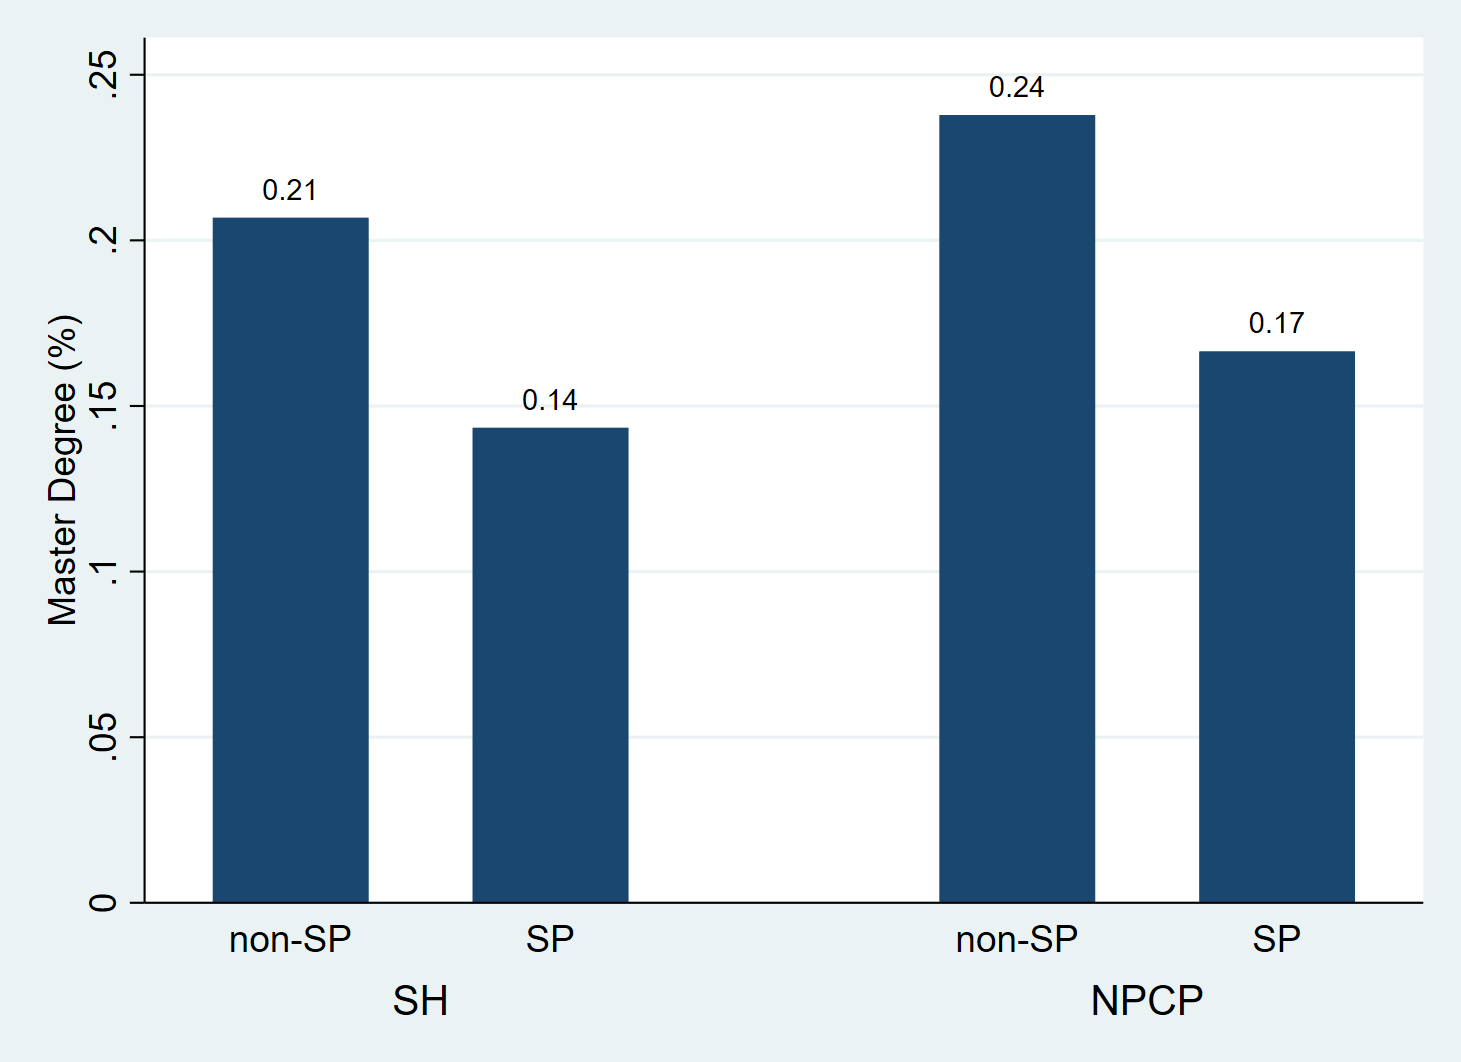
\includegraphics[scale=0.13]{master_sp.png}
        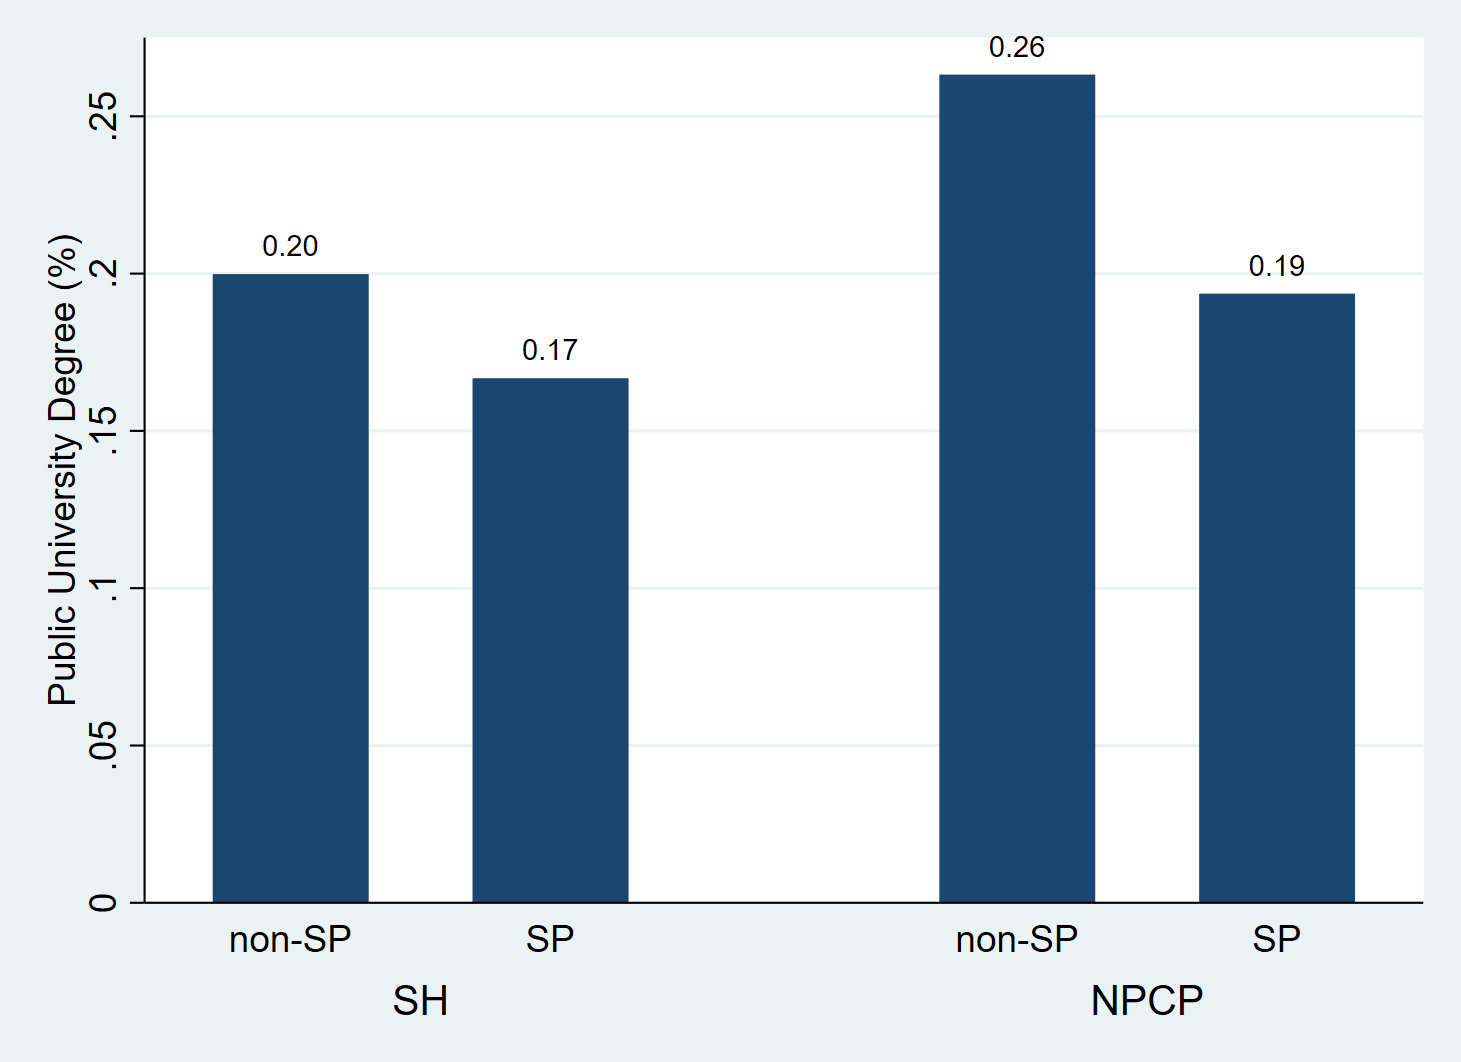
\includegraphics[scale=0.13]{public_sp.png}
    \end{figure}

    Finally, the comprehensive dataset also includes the survey data on their parent and teachers, in which the evaluation and observation on the children in their school age are detaily recorded.  We consider these dataset as the cure to omitted variable bias, so we look at each teacher's data thoroughly and pick out every potential confounding variable that either relates to treatment or outcome variable.  Besides, it's worth mentioning that since we want to reduce bias, we take great care not to include a covariate regarded as bad control by us.  As the following setup is done, we can proceed with the PDS analysis.


\section{Empirical Method} % Second paragraph: what's the assumption and the specification?

    The Post-Double Selection (PDS) method combining causal inference and machine learning is a very powerful and convenient method when we face this kind of huge and comprehensive dataset.  Normally, it's the curse of dimensionality problem we will encounter when we include more covariates and try to reduce the underlying omitted variable bias; however, the PDS method tackles this problem by introducing Lasso (Least Absolute Shrinkage and Selection Operator) and multi-stage regression.

    There are two assumptions supporting PDS method: conditional independence assumption and approximate sparsity, and three regression stages in PDS.  The first and second stage use Lasso to conduct regression on different dependent variable, that is, treatment variable and outcome variable, which can be formulated as below

    \begin{align}
    \text{SP}_i = \theta_0 + \sum_{i=1}^n \theta_j X_i^j + \lambda_\theta\sum_{i=1}^n \lvert \theta_j \rvert + \epsilon_i \\
    Y_i         = \eta_0   + \sum_{i=1}^n \eta_j X_i^j   + \lambda_\eta\sum_{i=1}^n \lvert \eta_j   \rvert + \delta_i
    \end{align}

    where the $X^j$ is the covariate we choose from the dataset, and $\{\lambda_\theta,\lambda_\eta\}$ are tuning parameters in the Lasso regression.  After the stages, we will have two different sets of selected covariates, denoted as $\Lambda_\theta,\ \Lambda_\eta$, and their union represents all the potential confounders.  So we can conduct the third stage OLS regression to identify the causal effect in the presence of CIA:

    \begin{align}
        Y_i = \beta_0 + \beta_{\text{PDS}}\text{SP}_i + \sum_{j \,\in\, \Lambda_\theta \cup \Lambda_\eta} \beta_j X_i^j + \epsilon_i
    \end{align}

    After we follow the same analysis process for each group, SH and CP, we obtain the estimated effect and discover the unexpected result which we will show in next part.


\section{Result}

    Accordingly, we perform the three different kinds of regression model, so as to gradually eliminate the omitted variable bias.  The first model is the single variable OLS, which gives us some interpretation of the correlation, the second model is the extension, where we add some controlled variables related to the student's background; and the last model is the PDS regression, where we include all the possible confounders and rely on machine's selection.  We should first show our result on the first outcome variable: university degree

    \begin{center}
    \begin{table}
    \caption{Regression on University for SH and CP group}
    \setlength{\tabcolsep}{0.5mm}
    \begin{tabular}{l*{6}c}
    \toprule
    &\multicolumn{3}{c}{SH} &\multicolumn{3}{c}{CP/NP} \\
    \cmidrule(l){2-4}\cmidrule(l){5-7}
    &\multicolumn{1}{c}{(1)}&\multicolumn{1}{c}{(2)}&\multicolumn{1}{c}{(3)}&\multicolumn{1}{c}{(4)}&\multicolumn{1}{c}{(5)}&\multicolumn{1}{c}{(6)} \\
    &\multicolumn{1}{c}{University}&\multicolumn{1}{c}{University}&\multicolumn{1}{c}{University}&\multicolumn{1}{c}{University}&\multicolumn{1}{c}{University}&\multicolumn{1}{c}{University} \\
    \midrule
    sp          &      -0.101\sym{***}&     -0.0284         &     -0.0165         &     -0.0340\sym{**} &     -0.0322\sym{**} &     -0.0264\sym{**} \\
        &     (0.000)         &     (0.109)         &     (0.340)         &     (0.011)         &     (0.015)         &     (0.041)         \\
    [1em]
    female      &                     &      0.0260\sym{**} &                     &                     &      0.0198\sym{***}&                     \\
        &                     &     (0.012)         &                     &                     &     (0.004)         &                     \\
    [1em]
    hs\_private  &                     &     -0.0850\sym{***}&     -0.0408\sym{***}&                     &     -0.0474\sym{***}&                     \\
        &                     &     (0.000)         &     (0.001)         &                     &     (0.000)         &                     \\
    [1em]
    hs\_urban    &                     &      0.0505\sym{***}&                     &                     &      0.0466\sym{***}&      0.0124         \\
        &                     &     (0.000)         &                     &                     &     (0.000)         &     (0.159)         \\
    [1em]
    general\_high&                     &       0.633\sym{***}&       0.538\sym{***}&                     &           0         &                     \\
        &                     &     (0.000)         &     (0.000)         &                     &         (.)         &                     \\
    [1em]
    paedu       &                     &       0.107\sym{***}&      0.0753\sym{***}&                     &      0.0448\sym{***}&      0.0330\sym{***}\\
        &                     &     (0.000)         &     (0.000)         &                     &     (0.000)         &     (0.000)         \\
    [1em]
    PDS\_control  &   &  &  Yes    &  &    &  Yes \\
    &   &      &      &   &      &      \\
    \hline
    \(N\)       &        5230         &        5230         &        5230         &        5766         &        5766         &        5766         \\
    \bottomrule
    \multicolumn{3}{l}{\footnotesize \textit{p}-values in parentheses} & \multicolumn{4}{r}{\footnotesize \sym{*} \(p<0.10\), \sym{**} \(p<0.05\), \sym{***} \(p<0.01\)}\\
    \end{tabular}
    \begin{tablenotes}
        The "PDS control" indicates whether we include covariates to perform PDS.  The number of total covariates we include is 98 for SH group, and 77 for CP group; the number of selected covariates is 22 for SH group, and 8 for CP group.
    \end{tablenotes}
    \end{table}
    \end{center}

    From Table 1, the single variable OLS result matches our intuition with a strong negative correlation between living in single parent family and obtaining university degree in future; however, it also shows that if we look at the PDS regression for the SH group, the causal relationship isn't significant, while it is for the CP group. This is the most interesting point in our analysis, because it's very peculiar as we expect the negative causal effect holds for these two different groups, but how does it differ?  We will explain when we dig deeper, that is, analyzing the other outcome variables.

    \begin{center}
    \begin{table}
    \caption{Regression on Master for SH and CP group}
    \setlength{\tabcolsep}{0.5mm}
    \begin{tabular}{l*{6}c}
    \toprule
    &\multicolumn{3}{c}{SH} &\multicolumn{3}{c}{CP/NP} \\
    \cmidrule(l){2-4}\cmidrule(l){5-7}
    &\multicolumn{1}{c}{(1)}&\multicolumn{1}{c}{(2)}&\multicolumn{1}{c}{(3)}&\multicolumn{1}{c}{(4)}&\multicolumn{1}{c}{(5)}&\multicolumn{1}{c}{(6)} \\
    &\multicolumn{1}{c}{Master}&\multicolumn{1}{c}{Master}&\multicolumn{1}{c}{Master}&\multicolumn{1}{c}{Master}&\multicolumn{1}{c}{Master}&\multicolumn{1}{c}{Master} \\
    \midrule
    sp          &     -0.0764\sym{***}&     -0.0530\sym{***}&     -0.0474\sym{***}&     -0.0635\sym{***}&     -0.0549\sym{***}&     -0.0465\sym{**} \\
        &     (0.000)         &     (0.001)         &     (0.003)         &     (0.001)         &     (0.005)         &     (0.015)         \\
    [1em]
    female      &                     &     -0.0873\sym{***}&     -0.0659\sym{***}&                     &      -0.111\sym{***}&     -0.0558\sym{***}\\
        &                     &     (0.000)         &     (0.000)         &                     &     (0.000)         &     (0.000)         \\
    [1em]
    hs\_private  &                     &     -0.0642\sym{***}&     -0.0343\sym{***}&                     &     -0.0494\sym{***}&                     \\
        &                     &     (0.000)         &     (0.004)         &                     &     (0.001)         &                     \\
    [1em]
    hs\_urban    &                     &      0.0424\sym{***}&                     &                     &      0.0833\sym{***}&      0.0570\sym{***}\\
        &                     &     (0.000)         &                     &                     &     (0.000)         &     (0.000)         \\
    [1em]
    general\_high&                     &       0.177\sym{***}&      0.0996\sym{***}&                     &           0         &                     \\
        &                     &     (0.000)         &     (0.000)         &                     &         (.)         &                     \\
    [1em]
    paedu       &                     &      0.0850\sym{***}&      0.0699\sym{***}&                     &       0.102\sym{***}&      0.0813\sym{***}\\
        &                     &     (0.000)         &     (0.001)         &                     &     (0.000)         &     (0.000)         \\
    [1em]
    PDS\_control  &   &  &  Yes    &  &    &  Yes \\
    &   &      &      &   &      &      \\
    \hline
    \(N\)       &        4848         &        4848         &        4848         &        5600         &        5600         &        5600         \\
    \bottomrule
    \multicolumn{3}{l}{\footnotesize \textit{p}-values in parentheses} & \multicolumn{4}{r}{\footnotesize \sym{*} \(p<0.10\), \sym{**} \(p<0.05\), \sym{***} \(p<0.01\)}\\
    \end{tabular}
    \begin{tablenotes}
        The "PDS control" indicates whether we include covariates to perform PDS.  The number of total covariates we include is 98 for SH group, and 77 for CP group; the number of selected covariates is 11 for SH group, and 8 for CP group.
        % puclic: SH is 16, CP is 20
    \end{tablenotes}
    \end{table}
    \end{center}

    In table 2, we see all the coefficients are significant under 1\% significant level, which indicates the effect is very strong.  As the PDS regression result shows, living in single parent family reduces the probability of obtaining master degree by 4\% and 4.6\%, respectively for SH and CP group.  We regard the impact as very prodigious and suggest that the underlying channels, economics situation and mental support, play a crucial role in the process.

    \begin{center}
    \begin{table}
    \caption{Regression on Public University for SH and CP group}
    \setlength{\tabcolsep}{0.5mm}
    \begin{tabular}{l*{6}c}
    \toprule
    &\multicolumn{3}{c}{SH} &\multicolumn{3}{c}{CP/NP} \\
    \cmidrule(l){2-4}\cmidrule(l){5-7}
    &\multicolumn{1}{c}{(1)}&\multicolumn{1}{c}{(2)}&\multicolumn{1}{c}{(3)}&\multicolumn{1}{c}{(4)}&\multicolumn{1}{c}{(5)}&\multicolumn{1}{c}{(6)} \\
    &\multicolumn{1}{c}{Public}&\multicolumn{1}{c}{Public}&\multicolumn{1}{c}{Public}&\multicolumn{1}{c}{Public}&\multicolumn{1}{c}{Public}&\multicolumn{1}{c}{Public} \\
    \midrule
    sp          &     -0.0468\sym{***}&     -0.0194\sym{*}  &     -0.0174\sym{*}  &     -0.0768\sym{***}&     -0.0739\sym{***}&     -0.0443\sym{**} \\
        &     (0.000)         &     (0.065)         &     (0.093)         &     (0.000)         &     (0.000)         &     (0.020)         \\
    [1em]
    female      &                     &      0.0197\sym{**} &                     &                     &     -0.0319\sym{**} &                     \\
        &                     &     (0.016)         &                     &                     &     (0.012)         &                     \\
    [1em]
    hs\_private  &                     &     -0.0870\sym{***}&     -0.0482\sym{***}&                     &      -0.182\sym{***}&     -0.0860\sym{***}\\
        &                     &     (0.000)         &     (0.000)         &                     &     (0.000)         &     (0.000)         \\
    [1em]
    hs\_urban    &                     &      0.0374\sym{***}&                     &                     &       0.131\sym{***}&      0.0968\sym{***}\\
        &                     &     (0.000)         &                     &                     &     (0.000)         &     (0.000)         \\
    [1em]
    general\_high&                     &       0.163\sym{***}&       0.137\sym{***}&                     &           0         &                     \\
        &                     &     (0.000)         &     (0.000)         &                     &         (.)         &                     \\
    [1em]
    paedu       &                     &      0.0664\sym{***}&      0.0464\sym{***}&                     &       0.110\sym{***}&      0.0641\sym{***}\\
        &                     &     (0.000)         &     (0.001)         &                     &     (0.000)         &     (0.000)         \\
    [1em]
    PDS\_control  &   &  &  Yes    &  &    &  Yes \\
    &   &      &      &   &      &      \\
    \hline
    \(N\)       &        5027         &        5027         &        5027         &        5576         &        5576         &        5576         \\
    \bottomrule
    \multicolumn{3}{l}{\footnotesize \textit{p}-values in parentheses} & \multicolumn{4}{r}{\footnotesize \sym{*} \(p<0.10\), \sym{**} \(p<0.05\), \sym{***} \(p<0.01\)}\\
    \end{tabular}
    \begin{tablenotes}
        The "PDS control" indicates whether we include covariates to perform PDS.  The number of total covariates we include is 98 for SH group, and 77 for CP group; the number of selected covariates is 16 for SH group, and 20 for CP group.
    \end{tablenotes}
    \end{table}
    \end{center}

    Now let's look at table 3, where the PDS regression result looks similar to the first table.  Compared with significantly negative impact for CP group, it's noticeable the impact nearly exist for SH group. So why is there an unneglected difference between these two group?  Since the only different characteristic for these groups is the year of birth, we suggest that the difference could be attributed to Taiwan's education reform in the 2000s, when the number of universities skyrocketed to raise people's general education level. 
    
    Although the reform has reduced the competition for children to enter university, we believe that the policy may widen the gap between those with good/bad economic condition, or in other words, living in single parent/nuclear family. The policy may do provide more opportunities for children to get into the university, but failing to cover the money shortage of those with bad economic condition, as a consequence, they would tend to suspend their educational investment after high school and enter labor market for finding work.  This sounds like a plausible story, with some evidence, we can make the argument more credible.

\section{Discussion and Conclusion}

    Overall, we find out that single parent family has the significant negative effect on academic degrees, especially in master degree. We also observe the different impact of single parent family. However, the channel is still unknown. The different effects between two groups might be related to the economic conditions of the students. 

    To confirm that the difference between SH and CP group is truely induced by family's economic background, we show another dependent variable -- $work\_year$ further. The variable $work\_year$ is defined as how many years these students enter the labor market when they are 25 years old. If single parent families do influence the students' economic situation, it is possible that students in single parent family will enter the labor market earlier, rather than getting the higher educational degree. Thus, we simply run the regression of single parent family on working year.

    In table 4, the single regression with some of our selected control variables shows that single parent families have significant effect on CP group, while it is not significant in SH group, which directly confirm our suppose about bad economic conditions in single parent families. Although the scale is only 0.2 years, we believe single parent families somehow force their children to enter the labor market earlier than general students, which might influence their highest level of education.
    \begin{center}
        \begin{table}
        \caption{Regression on Working Year for SH and CP group}
        \setlength{\tabcolsep}{0.5mm}
        \begin{tabular}{l*{4}c}
        \toprule
        &\multicolumn{2}{c}{SH} &\multicolumn{2}{c}{CP/NP} \\
        \cmidrule(l){2-3}\cmidrule(l){4-5}
        &\multicolumn{1}{c}{(1)}&\multicolumn{1}{c}{(2)}&\multicolumn{1}{c}{(3)}&\multicolumn{1}{c}{(4)}\\
        &\multicolumn{1}{c}{Work\_year}&\multicolumn{1}{c}{Work\_year}&\multicolumn{1}{c}{Work\_year}&\multicolumn{1}{c}{Work\_year}\\
        \midrule
        sp          &       0.257\sym{**} &       0.153         &       0.214\sym{***}&       0.200\sym{***}\\
                    &     (0.032)         &     (0.180)         &     (0.006)         &     (0.009)         \\
        [1em]
        female      &                     &      0.0312         &                     &       0.437\sym{***}\\
                    &                     &     (0.675)         &                     &     (0.000)         \\
        [1em]
        hs\_private  &                     &       0.380\sym{***}&                     &       0.139\sym{**} \\
                    &                     &     (0.000)         &                     &     (0.010)         \\
        [1em]
        hs\_urban    &                     &      -0.112\sym{*}  &                     &      -0.167\sym{***}\\
                    &                     &     (0.093)         &                     &     (0.000)         \\
        [1em]
        general\_high&                     &      -1.012\sym{***}&                     &           0         \\
                    &                     &     (0.000)         &                     &         (.)         \\
        [1em]
        paedu       &                     &      -0.400\sym{***}&                     &      -0.290\sym{***}\\
                    &                     &     (0.000)         &                     &     (0.000)         \\
        [1em]
        \_cons      &       2.959\sym{***}&       3.465\sym{***}&       2.940\sym{***}&       2.815\sym{***}\\
                    &     (0.000)         &     (0.000)         &     (0.000)         &     (0.000)         \\
        \hline
        \(N\)       &        2685         &        2685         &        3548         &        3548         \\
        \hline\hline
        \multicolumn{2}{l}{\footnotesize \textit{p}-values in parentheses} & \multicolumn{3}{r}{\footnotesize \sym{*} \(p<0.10\), \sym{**} \(p<0.05\), \sym{***} \(p<0.01\)}\\
        \end{tabular}
        \begin{tablenotes}
            We only run the simple regression with some control variables since the PDS method would drop most of the samples. The data quality doesn't allow us to utilize PDS method in this case.
        \end{tablenotes}
        \end{table}
        \end{center}
    Besides, our results are consistent with the previous paper.  \cite{Luoh2004}  also proves that the educational reform around 2000s does not benefit some economically vulnerable groups. He analyses the probability change of entering Taiwan universities. Due to the educational reform in 1987, the number of university in Taiwan abruptly increased. The total number of universities was 60 in 1995, but 135 in 2001, which allowed more students to attend the university.  \cite{Luoh2004} point out that when the proportion of school attendance is low, the increase of school opportunities will increase the influence of family background on the probability of individual school attendance, which means students from poor economic family will have more negative impact on the probability of attaining the bachelor degree. 
   
    In our case, single parent family do have some economic situation. The negative effect of single parent family was not really obvious until the educational reform enhanced the total probability of entering universities, which somehow crowded out the children from single parent family, making the coefficient of CP group to be significant. In other words, in Taiwan, after the reform amplified the total probability of entering university, the nagative impact of single parent family started to worsen.

    Some previous papers highlight the timeline of when parents divorced is also important. Unfortunately, the dataset we used can't covered this,so we just focus on children who ever go through the parent divorce experience. Another limitation is that we only provide the children's working year to support our assumption of bad economic conditions in single parent families. The future studies can dig into whether sociol capital channel also significantly affects the children's degree of education.



\section*{References}

% Remove or comment out the next two lines if you are not using bibtex.

\bibliography{reference}
\bibliographystyle{plain}



\end{document}

